\documentclass{article}
\usepackage{graphicx} % Required for inserting images
\usepackage{spverbatim}

\title{COMP1204 Coursework 2}
\author{Name: Andrew Milne - Username: am4n23 - Student ID: 34937188}
\date{17th May 2024}

\begin{document}

\maketitle

\tableofcontents

\newpage

\section{The Relational Model}

\subsection{EX1}

Since the initial table is too large to fit, I have cut it in half. "deaths" and "countriesAndTerritories" are next to each other.

\begin{table}[ht]
\centering
\begin{tabular}{|c|c|c|c|c|c|}
    \hline
    dateRep&day&month&year&cases&deaths\\
    (TEXT)&(INTEGER)&(INTEGER)&(INTEGER)&(INTEGER)&(INTEGER)\\
    \hline
    ...&...&...&...&...&...\\
    \hline
\end{tabular}
\caption{Initial table (left half)}
\label{StartTableLeft}
\end{table}

\begin{table}[ht]
\centering
\begin{tabular}{|c|c|c|c|c|}
    \hline
    countriesAndTerritories&geoId&countryterritoryCode&popData2020&continentExp\\
    (TEXT)&(TEXT)&(TEXT)&(INTEGER)&(TEXT)\\
    \hline
    ...&...&...&...&...\\
    \hline
\end{tabular}
\caption{Initial table (right half)}
\label{StartTableRight}
\end{table}

\subsection{EX2}

\begin{itemize}
\item dateRep $\rightarrow$ day
\item dateRep $\rightarrow$ month
\item dateRep $\rightarrow$ year
\item day, month, year $\rightarrow$ dateRep
\item dateRep,geoId $\rightarrow$ cases
\item dateRep,geoId $\rightarrow$ deaths
\item geoId $\rightarrow$ countriesAndTerritories
\item geoId $\rightarrow$ countryterritoryCode
\item countryterritoryCode $\rightarrow$ geoId
\item countriesAndTerritories $\rightarrow$ geoId
\item geoId $\rightarrow$ continentExp
\item geoId $\rightarrow$ popData2020
\end{itemize}

Assumptions:
\begin{itemize}
\item Each country has a unique countriesAndTerritories, geoId (as it seems to have been created specifically for this database) and countryterritoryCode.
\item cases and deaths are integers.
\item popData2020 contains a country's population data as of a single point in time, which is consistent throughout the data.
\item Each country is contained within a single continent. If a country was to be contained within multiple continents, contintentExp would see this as a unique single continent rather than multiple existing ones.
\item Empty values correspond to null rather than a known blank value.
\item Each dateRep corresponds to and is equivalent to the stated unique combination of day, month and year (e.g. when dateRep = "02/01/2020", day = 2, month = 1 and year = 2020, so dateRep will always be "02/01/2020" when day = 2, month = 1 and year = 2020). As a result, dateRep is unique for any given combination of day, month and year.
\item Unless representing cases and deaths, all values are non-nullable.
\item Text values are within the allowed length range in SQLite, and integer values are within the allowed value range in SQLite.
\item Key type is not important.
\item The text values are in British English and do not contain any spelling inconsistencies (e.g. "Europe" rather than "EUrope").
\end{itemize}

\subsection{EX3}
Possible candidate keys:
\begin{itemize}
\item \{day,month,year,geoId\}
\item \{day,month,year,countriesAndTerritories\}
\item \{day,month,year,countryterritoryCode\}
\item \{dateRep,geoId\}
\item \{dateRep,countriesAndTerritories\}
\item \{dateRep,countryterritoryCode\}
\end{itemize}

\subsection{EX4}

I have decided to use \{dateRep,geoId\}. This is split into two decisions:

\begin{itemize}
\item Whether to use day,month,year or dateRep. dateRep has been chosen as it is a single attribute.
\item Whether to use geoId, countriesAndTerritories or countryterritoryCode. This is a largely arbitrary decision, though the data in countriesAndTerritories seems to consistently be longer and can use underscores, which increases the potential for spelling inconsistencies, while this does not seem to be the case for geoId or countryterritoryCode. I am choosing to use geoId as it seems to be enforced that this value is 2 characters long, and its name implies that it is intended to be used as a primary key.
\end{itemize}

\section{Normalisation}

\subsection{EX5}

We have dateRep $\rightarrow$ day, month, year. We also have geoId $\rightarrow$ countriesAndTerritories, countryterritoryCode, continentExp, popData2020. As a result, the relation should be split into the following:

\begin{itemize}
\item A date relation, with primary key \{dateRep\}
\item A country relation, with primary key \{geoId\}
\item A COVID data relation, with primary key \{dateRep,geoId\}
\end{itemize}

Additionally, we need to consider what to do when further population data is added, so we also need to split popData2020 off into its own population relation, with primary key \{geoId\}. We assume that future population data will be added to this relation as a new attribute (e.g. as popData2021) due to the requirement that all existing column names are preserved.

\subsection{EX6}

As a result of EX5, I am creating the following relations ($\ref{DatesTable}$, $\ref{CountriesTable}$, $\ref{CovidTable}$ and $\ref{PopulationTable}$):

\begin{table}[ht]
\centering
\begin{tabular}{|c|c|c|c|}
    \hline
     \textbf{\textit{dateRep}}&day&month&year\\
     (TEXT)&(INTEGER)&(INTEGER)&(INTEGER)\\
     \hline
     ...&...&...&...\\
     \hline
\end{tabular}
\caption{Dates}
\label{DatesTable}
\end{table}

\begin{table}[ht]
\centering
\begin{tabular}{|c|c|c|c|}
    \hline
     \textbf{\textit{geoId}}&countriesAndTerritories&countryterritoryCode&continentExp\\
     (TEXT)&(TEXT)&(TEXT)&(TEXT)\\
     \hline
     ...&...&...&...\\
     \hline
\end{tabular}
\caption{Countries}
\label{CountriesTable}
\end{table}

\begin{table}[ht]
\centering
\begin{tabular}{|c|c|c|c|}
    \hline
     \textbf{\textit{dateRep}}&\textbf{\textit{geoId}}&cases&deaths\\
     (TEXT)&(TEXT)&(INTEGER)&(INTEGER)\\
     \hline
     ...&...&...&...\\
     \hline
\end{tabular}
\caption{CovidData}
\label{CovidTable}
\end{table}

\begin{table}[ht]
\centering
\begin{tabular}{|c|c|}
    \hline
     \textbf{\textit{geoId}}&popData2020\\
     (TEXT)&(INTEGER)\\
     \hline
     ...&...\\
     \hline
\end{tabular}
\caption{CountryPopulationByYear}
\label{PopulationTable}
\end{table}

The primary key for each table is in bold italics. If multiple attributes in a single table are in bold italics, they are part of a composite key.

\subsection{EX7}

In the functional dependencies below, bold attributes are key attributes, while a group of bold-italic attributes is a super key.\newline

In $\ref{DatesTable}$:
\begin{itemize}
\item \textbf{\textit{dateRep}} $\rightarrow$ day
\item \textbf{\textit{dateRep}} $\rightarrow$ month
\item \textbf{\textit{dateRep}} $\rightarrow$ year
\item day,month,year $\rightarrow$ \textbf{\textit{dateRep}}
\end{itemize}

This table contains no transitive dependencies.\newline

In $\ref{CountriesTable}$:
\begin{itemize}
\item \textbf{\textit{geoId}} $\rightarrow$ countriesAndTerritories
\item \textbf{\textit{geoId}} $\rightarrow$ countryterritoryCode
\item \textbf{\textit{geoId}} $\rightarrow$ continentExp
\item countriesAndTerritories $\rightarrow$ \textbf{\textit{geoId}}
\item countryterritoryCode $\rightarrow$ \textbf{\textit{geoId}}
\end{itemize}

This table contains no transitive dependencies.\newline

In $\ref{CovidTable}$:
\begin{itemize}
\item \textbf{\textit{dateRep,geoId}} $\rightarrow$ cases
\item \textbf{\textit{dateRep,geoId}} $\rightarrow$ deaths
\end{itemize}

This table contains no transitive dependencies.\newline

\newpage
In $\ref{PopulationTable}$:
\begin{itemize}
\item \textbf{\textit{geoId}} $\rightarrow$ popData2020
\end{itemize}

This table contains no transitive dependencies.\newline

As a result, there are no transitive dependencies present.

\subsection{EX8}

There are no transitive dependencies present in this system, and we already know this system is in 2NF, therefore we now know that it is in 3NF.

\subsection{EX9}

The candidate keys for each table are as follows:\newline

In $\ref{DatesTable}$:
\begin{itemize}
\item \{dateRep\}
\item \{day,month,year\}
\end{itemize}

In $\ref{CountriesTable}$:
\begin{itemize}
\item \{geoId\}
\item \{countriesAndTerritories\}
\item \{countryterritoryCode\}
\end{itemize}

In $\ref{CovidTable}$:
\begin{itemize}
\item \{dateRep,geoId\}
\end{itemize}

In $\ref{PopulationTable}$:
\begin{itemize}
\item \{geoId\}
\end{itemize}

All functional dependencies (as seen in EX7) have a candidate key as their determinant, and we know this system is in 3NF, therefore we now know this it is in BCNF (aka 3.5NF).

\section{Modelling}

\subsection{EX10}

To set up the initial database, I did the following:
\begin{itemize}
\item I added a new PATH system variable to my computer, specifically to the location of my \verb|sqlite-tools-win-x64-3450200| folder.
\item I navigated to my \verb|Coursework 2| folder in my command prompt, which I ran \verb|sqlite3 coronavirus.db| from to create a new coronavirus database.
\item I imported the dataset csv to the database by using \verb|.import --csv dataset.csv dataset|.
\item I output the database as a \verb|.sql| file by using \verb|.output dataset.sql|.
\item I dumped the output to my \verb|Coursework 2| folder by using \verb|.dump|.
\end{itemize}

\subsection{EX11}

I have created the full normalised representation, which uses the relations specified in the Normalisation section.

I am using dateRep and geoId as my primary key attributes, but it should be noted that they act as surrogate keys, uniquely representing dates and countries respectively, even though I have not introduced them personally.

Indexes are created, but only for enforcing the primary keys and UNIQUE constraints, and this is done automatically when creating them.

Three foreign keys are being used: dateRep and geoId in CovidData, to ensure that it does not reference invalid dates or countries (something which would could errors when joining the tables), and geoId in CountryPopulationByYear, to ensure that only valid countries are referenced (in order to act as a minor safeguard against incorrect data allocation and to prevent redundant data).

\subsection{EX12}

I have populated these tables by using the previously created database (in EX10). 

\subsection{EX13}

I have run the following with no coronavirus.db file existing:

\begin{spverbatim}
sqlite3 coronavirus.db < dataset.sql
sqlite3 coronavirus.db < ex11.sql
sqlite3 coronavirus.db < ex12.sql
\end{spverbatim}

This failed the first time I attempted this, as the \verb|UNIQUE| constraints were violated. Upon updating ex12.sql so that the \verb|SELECT| statements were followed by \verb|DISTINCT| (and deleting the coronavirus.db file created by dataset.sql and ex11.sql), I was able to execute all three commands successfully.

\newpage
\section{Querying}

\subsection{EX14}

\textbf{Command(s) used:}
\begin{spverbatim}
SELECT SUM(cases),SUM(deaths)
FROM CovidData;
\end{spverbatim}

\textbf{Description of approach:}
The aggregation function \verb|SUM| was created exactly for scenarios like this - it automatically calculates and returns the sum of all values in the requested column (if \verb|WHERE| is included, all values that match the specified condition). Using it on \verb|cases| and \verb|deaths| without any conditions was all that was required.

\subsection{EX15}

\textbf{Command(s) used:}
\begin{spverbatim}
SELECT CovidData.dateRep,cases
FROM CovidData
    JOIN Dates
        ON CovidData.dateRep = Dates.dateRep
    JOIN Countries
        ON CovidData.geoId = Countries.geoId
WHERE countriesAndTerritories='United_Kingdom'
ORDER BY year,month,day;
\end{spverbatim}

\textbf{Description of approach:}
I broke this into two sections: \verb|SELECT (...) WHERE| and \verb|ORDER BY|. For the first, I initially had it just select \verb|dateRep| and \verb|cases| where \verb|geoId|='UK', but later realised that it would be more appropriate to inner join with \verb|Countries| so that the condition could be based on \verb|countriesAndTerritories|, as the exercise was requesting the United Kingdom, not just the \verb|geoId| of 'UK'. For the second, I needed to inner join with \verb|Dates| so that it could be ordered by \verb|year|, \verb|month| and \verb|day|. It was done in this order due to how \verb|ORDER BY| works - it sorts by \verb|year|, then it sorts each \verb|year| individually by \verb|month|, then it sorts each \verb|year|-\verb|month| combination individually by \verb|day|.

\subsection{EX16}

\textbf{Command(s) used:}
\begin{spverbatim}
SELECT countriesAndTerritories,CovidData.dateRep,cases,deaths
FROM CovidData
    JOIN Dates
        ON CovidData.dateRep = Dates.dateRep
    JOIN Countries
        ON CovidData.geoId = Countries.geoId
ORDER BY continentExp,Countries.geoId,year,month,day;
\end{spverbatim}

\textbf{Description of approach:}
The exercise asked for the country name, so \verb|countriesAndTerritories| was used once again, which required a join with \verb|Countries|. In future version of this data set, it is likely that additional continents would be added, so I ordered by continent before \verb|geoId| (I used the version on \verb|Countries| for consistency, and ordered by \verb|geoId| as it essentially acts as a surrogate key). The ordering by date is identical to EX15:
\begin{quote}
I needed to inner join with \verb|Dates| so that it could be ordered by \verb|year|, \verb|month| and \verb|day|. It was done in this order due to how \verb|ORDER BY| works - it sorts by \verb|year|, then it sorts each \verb|year| individually by \verb|month|, then it sorts each \verb|year|-\verb|month| combination individually by \verb|day|.
\end{quote}

\subsection{EX17}

\textbf{Command(s) used:}
\begin{spverbatim}
SELECT countriesAndTerritories AS 'Country Name',ROUND((CAST(SUM(cases) AS REAL)/NULLIF(popData2020,0))*100,2) AS '% Cases of Population',ROUND((CAST(SUM(deaths) AS REAL)/NULLIF(popData2020,0))*100,2) AS '% Deaths of Population'
FROM CovidData
    JOIN Countries
        ON Countries.geoId = CovidData.geoId
    JOIN CountryPopulationByYear
        ON Countries.geoId = CountryPopulationByYear.geoId
GROUP BY Countries.geoId;
\end{spverbatim}

\textbf{Description of approach:}
As standard, \verb|countriesAndTerritories| (requiring a join with \verb|Countries|) was used for the country names. \verb|CountryPopulationByYear| was also required to be joined, as the statistics here were requested as a percentage of the countries' total populations. I also rounded the percentages to 2 decimal places, but due to the division had to cast the numerators to real and use \verb|NULLIF| to handle potential division by zero. I also had to group by \verb|geoId| in order to prevent all the resulting percentages from being summed together.

\subsection{EX18}

\textbf{Command(s) used:}
\begin{spverbatim}
SELECT countriesAndTerritories AS 'Country Name',ROUND((CAST(SUM(deaths) AS REAL)/NULLIF(CAST(SUM(cases) AS REAL),0))*100,2) AS '% Deaths of Country Cases'
FROM CovidData
    JOIN Countries
        ON CovidData.geoId = Countries.geoId
GROUP BY Countries.geoId
ORDER BY 2 DESC
LIMIT 10;
\end{spverbatim}

\textbf{Description of approach:}
As in EX17, \verb|countriesAndTerritories| was used for the country names again, requiring a join with \verb|Countries|, grouping was done by \verb|geoId| in order to prevent all the resulting percentages from being summed together and the percentage calculations involved casting the numerator to real, using \verb|NULLIF| to prevent a division by zero and rounding to 2 decimal places. On top of this, I ordered by the second column (the calculated statistic) in a descending order, which I also used alongside the limit of 10 in order to restrict the result to the requested top 10.

\subsection{EX19}

\textbf{Command(s) used:}
\begin{spverbatim}
    SELECT CovidData.dateRep,SUM(deaths) OVER upToHere AS 'Cumulative UK Deaths',SUM(cases) OVER upToHere AS 'Cumulative UK Cases'
    FROM CovidData
        JOIN Dates
            ON CovidData.dateRep = Dates.dateRep
        JOIN Countries
            ON CovidData.geoId = Countries.geoId
    WHERE countriesAndTerritories='United_Kingdom'
    WINDOW upToHere AS (ORDER BY year,month,day ROWS BETWEEN UNBOUNDED PRECEDING AND CURRENT ROW)
    ORDER BY year,month,day;
\end{spverbatim}

\textbf{Description of approach:}
As usual, \verb|countriesAndTerritories| was used for the country names, but it was also used this time to filter for just the United Kingdom. \verb|geoId| could be used instead, but I chose this way because a user may not know what \verb|geoId| corresponds to which country. I also used a window "\verb|upToHere|" in order to restrict the sums of \verb|cases| and \verb|deaths| to the date mentioned and prior, which required a join with \verb|Dates|.

\section{Extension}

\subsection{EX20}
\textbf{Description of approach:}\newline

\textit{SQLite3:}
As always, I used \verb|countriesAndTerritories| to represent the country (which required a join with \verb|Countries|). I used a nested \verb|SELECT| statement (which uses grouping by \verb|geoId| and descending ordering by sum of deaths with limit 10) within a \verb|WHERE| in order to restrict the output to the top 10 countries for deaths within the data. Additionally, I used a \verb|WINDOW| to get the death total to be just the total for that country (using partition) for the date being considered and earlier (using order, which required a join with \verb|Dates| and also ensured the output data was in chronological order, and the "\verb|ROWS BETWEEN UNBOUNDED|..." statement). I then exported this to a temporary \verb|csv| file. Each row of the resulting file contains the country being considered in the leftmost column, followed by (going left to right) the date being considered and the cumulative deaths for this country from the start of its data to that row's date.\newline

\textit{Bash Script (Preparing for GnuPlot):}
I started by creating a variable "\verb|countries|", using \verb|cat| and \verb|awk| to have it hold a list of the countries in the temporary \verb|csv| file. I then created an array of 10 strings, each of which was made to hold every date the string's corresponding country has data for (i.e. the first country for the first array element, etc.) and the cumulative deaths for that country on that date. These strings are then iterated through in order to create an individual array for each country, the elements of which are equivalent to the non-country data for a single row of the \verb|csv| file (though each array only contains the data for a single country, which is their corresponding one as mentioned earlier). This results in, for example, a row of "\verb|Country-a,01/01/2021,5|" becoming "\verb|01/01/2021,5|" as an element of \verb|CovidData1|, assuming that "\verb|Country-a|" is the first country to appear in the array. The chronological order of data within countries is also preserved.\newline

\textit{GnuPlot:}
The GnuPlot code starts with some setup commands, which set up the graphics for the output file, register the comma as the separating value and ensures that the strings representing time are recognised. Following this, I copy the arrays created in the Bash Script section into GnuPlot arrays (which have a defined size, unlike bash arrays). Finally, I plot the graph, using the left column (date) as the x axis and right column (cumulative deaths) as the y axis - each line of code creates a set of points corresponding to a single distinct country (with these points being a single colour, which is distinct for each country). The "\verb|t system()|" portions of the plot command lines create the legend, as the "\verb|countries|" variable from the Bash Script section is used to show which line represents which country. To complete the graph, "\verb|with lines|" draws a line between all of the points that line of code creates (of the same colour as those points).

\newpage
\section{Appendix}
\subsection{EX20 Full Script}
\begin{spverbatim}
#!/bin/sh

#Note: This has been tested using SQLite 3.45.2, gnuplot 6.0 patchlevel 0 and GNU bash 4.2.46(2)-release. Running this on earlier versions of these software may cause unintended errors.

#SQLite3 Commands
sqlOutput=$(mktemp --suffix=.csv)
sqlite3 coronavirus.db "SELECT DISTINCT Countries.countriesAndTerritories,
CovidData.dateRep,TOTAL(CovidData.deaths) OVER upToHere AS 'CumulativeDeaths' \
FROM CovidData \
        JOIN Dates \
                ON CovidData.dateRep = Dates.dateRep \
        JOIN Countries \
                ON CovidData.geoId = Countries.geoId \
WHERE CovidData.geoId IN (SELECT geoId \
        FROM CovidData \
        GROUP BY geoId \
        ORDER BY SUM(deaths) DESC \
        LIMIT 10) \
WINDOW upToHere AS (PARTITION BY CovidData.geoId ORDER BY year,month,day ROWS BETWEEN UNBOUNDED PRECEDING AND CURRENT ROW) \
ORDER BY CovidData.geoId,year,month,day;" > $sqlOutput

#Set up for GnuPlot
countries=$(cat $sqlOutput | awk -F, '{print $1}' | sort | uniq)
CovidData=()
for i in $(seq 1 10)
do
    relevantCountry=$(echo "$countries" | tail -n+$i | head -1)
    CovidData[$i]=$(awk -F, -v nation="$relevantCountry" '{if ($1 == nation) {print $2 "," $3}}' $sqlOutput)
    eval "CovidData$i=()"
    arraylength=1;
    for group in ${CovidData[$i]}
    do
        eval "CovidData$i[$arraylength]=$group";
        let arraylength=arraylength+1;
    done
done


#GnuPlot Commands
gnuplot<<ENDOF-GNUPLOT
set terminal png truecolor
set output "graph.png"
set datafile separator ","
set xdata time
set timefmt '%d/%m/%Y'
set xrange ["31/12/2019":"04/05/2022"]
set yrange [0:180000]
set format x "%m/%y"
unset x2tics
unset y2tics

size1 = system("echo ${#CovidData1[*]}")
array data1[size1]
do for [i=1:size1] {data1[i] = ${CovidData1[i]}}

size2 = system("echo ${#CovidData2[*]}")
array data2[size2]
do for [i=1:size2] {data2[i] = ${CovidData2[i]}}

size3 = system("echo ${#CovidData3[*]}")
array data3[size3]
do for [i=1:size3] {data3[i] = ${CovidData3[i]}}

size4 = system("echo ${#CovidData4[*]}")
array data4[size4]
do for [i=1:size4] {data4[i] = ${CovidData4[i]}}

size5 = system("echo ${#CovidData5[*]}")
array data5[size5]
do for [i=1:size5] {data5[i] = ${CovidData5[i]}}

size6 = system("echo ${#CovidData6[*]}")
array data6[size6]
do for [i=1:size6] {data6[i] = ${CovidData6[i]}}

size7 = system("echo ${#CovidData7[*]}")
array data7[size7]
do for [i=1:size7] {data7[i] = ${CovidData7[i]}}

size8 = system("echo ${#CovidData8[*]}")
array data8[size8]
do for [i=1:size8] {data8[i] = ${CovidData8[i]}}


size9 = system("echo ${#CovidData9[*]}")
array data9[size9]
do for [i=1:size9] {data9[i] = ${CovidData9[i]}}

size10 = system("echo ${#CovidData10[*]}")
array data10[size10]
do for [i=1:size10] {data10[i] = ${CovidData10[i]}}

plot data1 using 1:2 t system("echo $countries | tail -n+1 | head -1") with lines, \
data2 using 1:2 t system("echo $countries | tail -n+2 | head -1") with lines, \
data3 using 1:2 t system("echo $countries | tail -n+3 | head -1") with lines, \
data4 using 1:2 t system("echo $countries | tail -n+4 | head -1") with lines, \
data5 using 1:2 t system("echo $countries | tail -n+5 | head -1") with lines, \
data6 using 1:2 t system("echo $countries | tail -n+6 | head -1") with lines, \
data7 using 1:2 t system("echo $countries | tail -n+7 | head -1") with lines, \
data8 using 1:2 t system("echo $countries | tail -n+8 | head -1") with lines, \
data9 using 1:2 t system("echo $countries | tail -n+9 | head -1") with lines, \
data10 using 1:2 t system("echo $countries | tail -n+10 | head -1") with lines
ENDOF-GNUPLOT
\end{spverbatim}

\hfill \break
(Note: two blank lines returns were added to this code relative to the .sh file submitted. These are within two existing spaces between code, one new line in each location, in order to better format it within the pages of this \LaTeX document. Additionally, in order for the first line of the sqlite3 command to fit within the page, it has been cut in half by a carriage return after "Countries.countriesAndTerritories" for readability purposes. This is not present in the submitted .sh file.)

\newpage
\subsection{EX20 Final Graph}
\begin{figure}[ht]
    \centering
    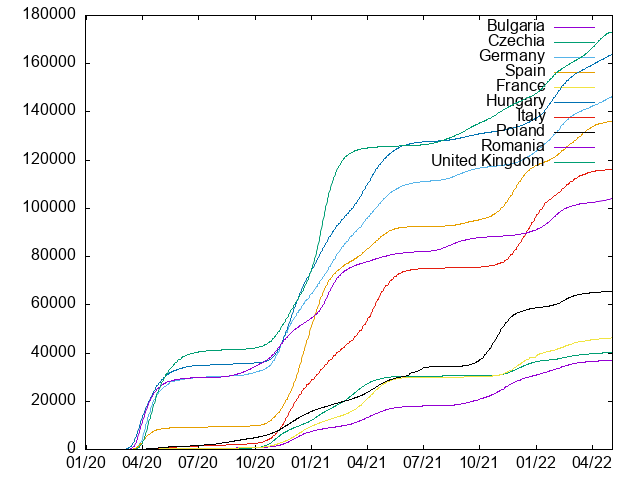
\includegraphics[width=1\linewidth]{graph.png}
    \caption{The graph created using the code shown in the "EX20 Full Script" subsection of the Appendix.}
    \label{fig:extension-graph}
\end{figure}

\end{document}